% Declare experimental floats early so they accompany the results, before Conclusion.

\begin{table*}[!t]
  \centering
  \caption{\textbf{Goal-conditioned planning with CEM.} Zhou et al.~\cite{zhou2024dinowm} evaluate PushObj on two unseen shapes. Our PushObj evaluation covers seven shapes, including three unseen during pretraining. PushT covers six shifts, including three recolorings. Success is in percent. Steps is the mean replan count, with failures counted as 30. Rope and granular report Chamfer distance. Italics denote published results; bold compares the matched methods below the rule. $^{\mathrm{o}}$: offline PushT adapter; $^{\mathrm{T}}$: T-only checkpoint in our rigid-object runs.}
  \label{tab:main}
  \small
  \setlength{\tabcolsep}{3.5pt}
  \begin{tabular}{@{}lccccccccc@{}}
    \toprule
    & PushObj~\cite{zhou2024dinowm} & \multicolumn{3}{c}{PushObj (this study)} & \multicolumn{3}{c}{PushT visual shifts} & Rope & Granular\\
    \cmidrule(lr){2-2}\cmidrule(lr){3-5}\cmidrule(lr){6-8}\cmidrule(lr){9-9}\cmidrule(lr){10-10}
    Method & Unseen (2) $\uparrow$ & All (7) $\uparrow$ & Unseen (3) $\uparrow$ & Steps $\downarrow$
      & Shift (6) $\uparrow$ & Color (3) $\uparrow$ & Steps $\downarrow$ & CD $\downarrow$ & CD $\downarrow$\\
    \midrule
    \inputrows{tables/main_rows.tex}
    \bottomrule
  \end{tabular}
\end{table*}

\begin{figure*}[!t]
  \centering
  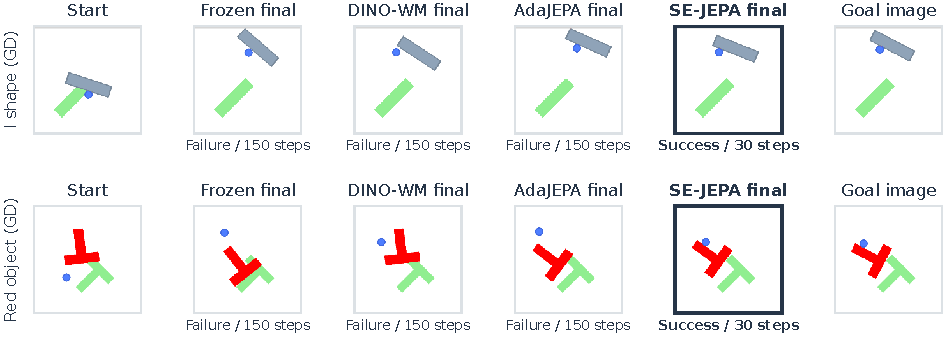
\includegraphics[width=\textwidth]{qualitative.pdf}
  \caption{\textbf{Persistent memory resolves failures of episodic adaptation.} Selected GD examples on an unseen I shape (top) and red-object shift (bottom). Frozen and AdaJEPA exhaust 30 replans in both cases; \textbf{\ours} succeeds in six and seven, respectively. Each row shares the same start and goal. The goal image specifies the pusher position and object pose; the green marker is static.}
  \label{fig:qualitative}
\end{figure*}

\begin{figure*}[!t]
  \centering
  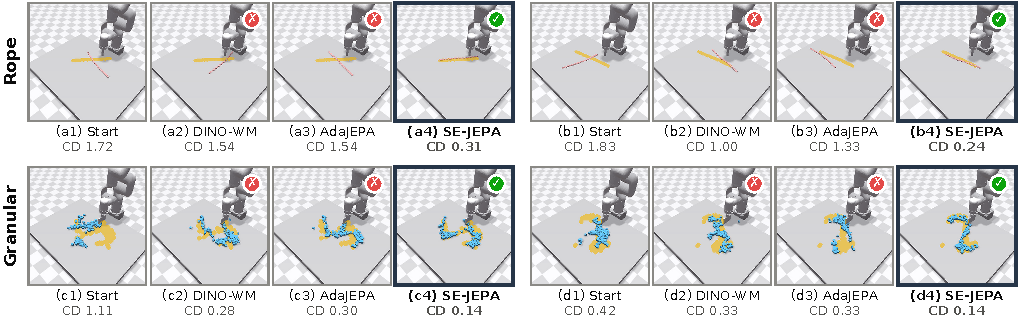
\includegraphics[width=\textwidth]{deform_qualitative.pdf}
  \caption{\textbf{Consolidated predictions support deformable manipulation.} Real FleX simulator trajectories for rope (top) and granular material (bottom), with two instances per task. Each group shows the start and the three methods' final states after 15 pushes; gold denotes the goal. These third-pass examples illustrate successful slow-only consolidation and were selected where both baselines fail. Frozen DINO-WM frames replay its executed actions. The aggregate fourth-pass results are reported in Table~\ref{tab:main}.}
  \label{fig:deform_qualitative}
\end{figure*}

\begin{figure}[!t]
  \centering
  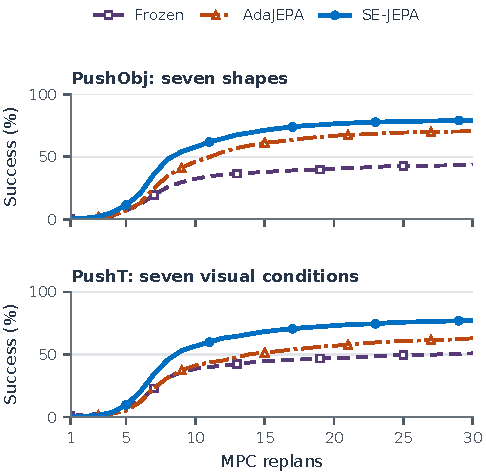
\includegraphics[width=\linewidth]{planning_efficiency.pdf}
  \caption{\textbf{Higher success within the same interaction budget.} Cumulative held-out success under CEM. Curves use all seven shapes (top) and all seven visual conditions (bottom).}
  \label{fig:efficiency_main}
\end{figure}

\begin{figure}[!t]
  \centering
  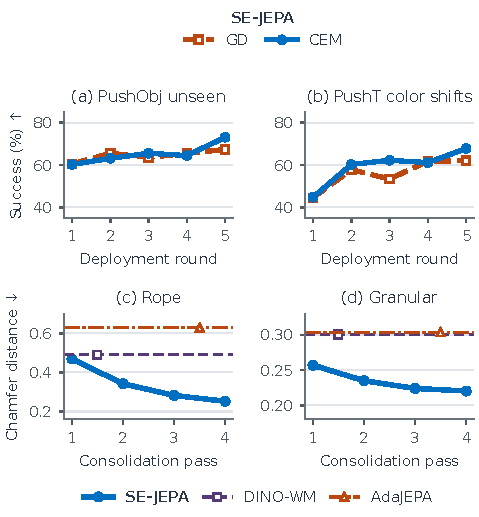
\includegraphics[width=\linewidth]{learning_progress.pdf}
  \caption{\textbf{Deployment experience improves two backbone families.} Top: ResNet-based models, with five rounds of online success on unseen PushObj shapes and three PushT color shifts; curves average three learning chains with targets resampled each round. Bottom: DINO-WM, with four consolidation passes over 50 fixed rope or granular instances; curves show mean CD. The horizontal lines are frozen DINO-WM and AdaJEPA.}
  \label{fig:deployment}
\end{figure}
